\documentclass[10pt,a4paper]{report}
\usepackage[utf8]{inputenc}
\usepackage{amsmath}
\usepackage{amsfonts}
\usepackage{amssymb}
\usepackage{fancyhdr}
\usepackage{tikz}

\usetikzlibrary{positioning, arrows, backgrounds, fit, shapes}
\usepackage{titlesec, blindtext, color}
\newcommand{\hsp}{\hspace{20pt}}
\titleformat{\chapter}[hang]{\Huge\bfseries}{\thechapter\hsp}{0pt}{\Huge\bfseries}

\newcommand{\attr}{\vspace{1ex} \hrule \vspace{1ex}}

\begin{document}
\chapter{Augmented Chess:\\ Assignment 8}

\begin{center}
{\Large \textbf{Group Members}}

\begin{tabular}{l r}
Jacob Holm Mortensen            &       jmorte14@student.aau.dk\\
Martin Raunkjær Andersen        &       marand13@student.aau.dk\\
Thomas Gwynfryn McCollin        &       tmccol14@student.aau.dk
\end{tabular}
\end{center}

\section{Question 1}
\begin{quote}
\textit{From the Interface Design Patterns presented in "User interface design practices in simple single page web applications", which ones are used in your application? For those that are used, indicate the concrete implementation used. For those that are not used but that are possible to use, how could they be included to enhance the user interface of your Web application?}
\end{quote}
Bear in mind that some of the functionality described in this section is not implemented yet, the section describes the finished product or the design.


The application makes additional information available to the user when a piece is selected. This information consists of the pieces attributes as well as the possible valid moves. This is consistent with the details on demand interface design pattern. The pattern has been implemented as a attribute box which shows the currently selected pieces attributes, the box is always visible, but the content changes based on the selected unit. Furthermore the legitimate moves that a piece can make are illustrated as highlighted cells on the chess board, these are only visible when a piece is selected.


When the user is managing their armies their attention is focused on using a number of input fields and some confirmation pop-ups. The fields are used to modify the attributes of the army pieces and the pop-ups are used when committing changes. A change could changing the name of an army or finalising the modification of an army.


The application presents the user with all possible actions at any given moment. During the game each piece represents a different course of action and when managing armies, the user is faced with a rich user interface. To counteract the increased complexity of this, the application functionality is as simplified as possible. The most complex operations of application are present when managing armies, this interface consists of a large array of different buttons and input fields. This is consistent with multifunction control.


Finally actions on demand and user driven page component visibility interface patterns could be included in the application. The user driven page component visibility pattern is circumvented by the different dynamic pages generated on the client side. This effectively only shows the relevant information, but this is not directly controlled by the user. The actions on demand pattern could be used instead of the multifunction control, however hiding functionality from the users would not benefit the application in this case.
\section{Question 2}
\begin{quote}
\textit{Consider the advantages and disadvantages of implementing your Web application as a single page application. In which context, would it be better to implement it as a single page application?}
\end{quote}

The Augment Chess application is a single page application. The advantages of single page applications outweighs the disadvantages, in the case of Augment Chess. Single page applications allow for more reuse of code than multi page applications. This reduces development complexity.
Since most rendering logic is performed client side, less strain is put on the server, allowing us to server more users. In a single page application multiple view templates and component resources are downloaded initially. This means that the single page application is more "snappy" or fast than a multi page application, since less calls are made to the server while using the page, which is important for usability and user satisfaction. This also further reduces server strain. Furthermore, single page application can use the the same origin pattern to enforce greater security. The reason that this is easier in multi page applications is that the routing component knows all valid sites beforehand, this is the case because valid sites are local or share origin with the application.
The disadvantages of single page applications consist of a large initial download and a much greater memory consumption. The full application must be downloaded initially and the application must be kept in memory throughout use. Furthermore, the single page application only has one page and therefore a single point of failure. Should something go wrong with the page, the entire application is dysfunctional whereas a multi page application could still serve the remaining pages properly regardless of a single broken page.

\section{Question 3}
\begin{quote}
\textit{Use the UML model presented in "A Model-Driven Development of Web Applications Using AngularJS Framework" to model your Web application (or a single page application version of your Web application if you are not implementing a single page application)}
\end{quote}

The following UML diagram describes the Augment Chess application. The UML is very cluttered, this is due to the size of the diagram and that it has been confined to a single page.

\makebox[\textwidth][c]{
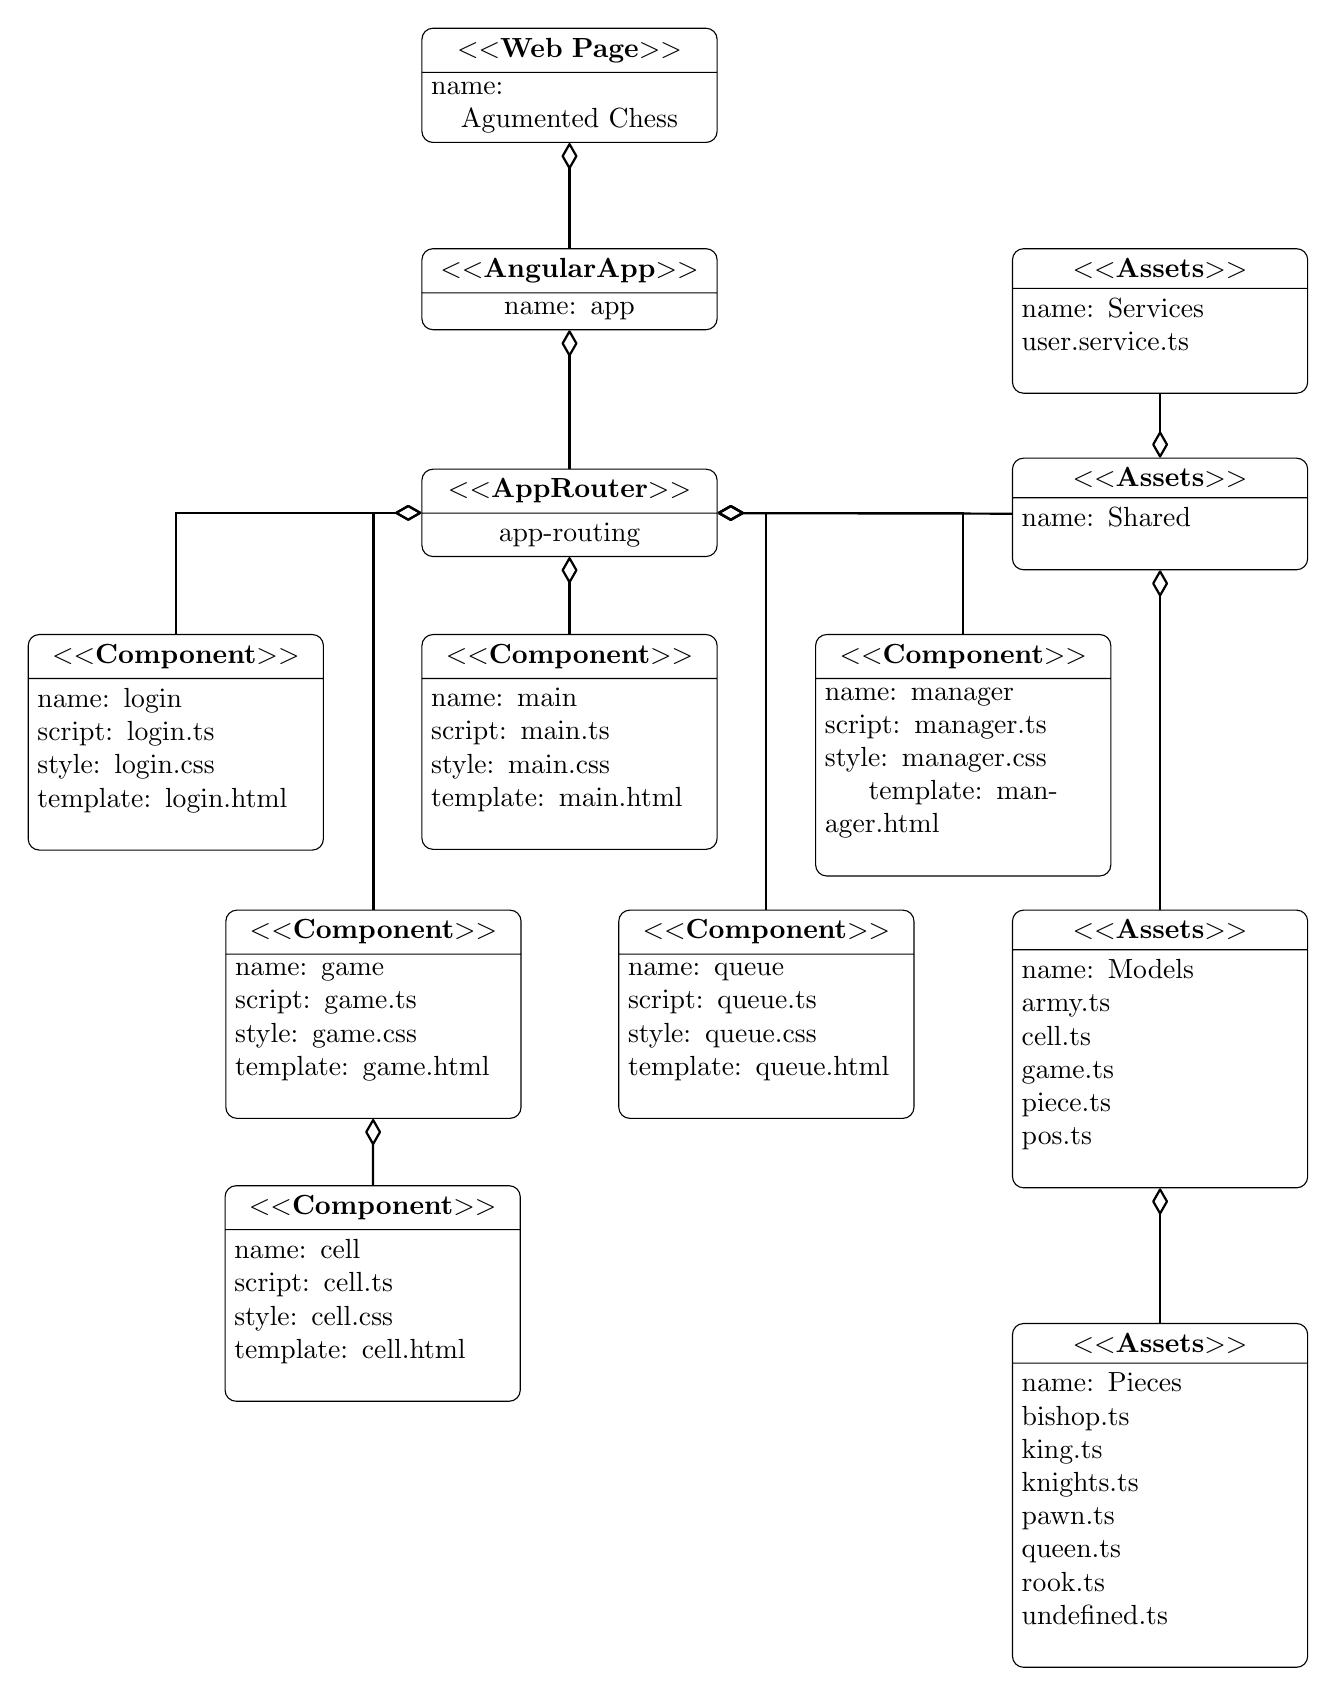
\begin{tikzpicture}
\tikzstyle{class}=[rectangle, draw=black, rounded corners, rectangle split, , rectangle split parts=2,
        text centered, anchor=north, text=black, text width=10em]
\tikzstyle{inherit}=[->, >=open triangle 90, thick]
\tikzstyle{line}=[-, thick]
\tikzstyle{aggregate}=[->, >=open diamond, thick]

\def \x {5}
\def \y {-3.5}    

    \node (page) [class] at (0,0.8*\y){
            \textbf{$<<$Web Page$>>$}
            \nodepart{second}name:\newline
            Agumented Chess
    };
    
    \node (app) [class] at (0,1.6*\y){
            \textbf{$<<$AngularApp$>>$}
            \nodepart{second}name: app
    };
    
    \node (rout) [class] at (0,2.4*\y){
            \textbf{$<<$AppRouter$>>$}
            \nodepart{second}app-routing
    };
    
	\node (serv) [class] at (1.5*\x,1.6*\y){
            \textbf{$<<$Assets$>>$}
            \nodepart{second}name: Services\newline
            user.service.ts\newline
    };    
    
    \node (share) [class] at (1.5*\x,2.36*\y){
            \textbf{$<<$Assets$>>$}
            \nodepart{second}name: Shared\newline
    };
    
    \node (mod) [class] at (1.5*\x,4*\y){
            \textbf{$<<$Assets$>>$}
            \nodepart{second}name: Models\newline
            army.ts\newline
            cell.ts\newline
            game.ts\newline
            piece.ts\newline
            pos.ts\newline
    };
    
    \node (pieces) [class] at (1.5*\x,5.5*\y){
            \textbf{$<<$Assets$>>$}
            \nodepart{second}name: Pieces\newline
            bishop.ts\newline
            king.ts\newline
            knights.ts\newline
            pawn.ts\newline
            queen.ts\newline
            rook.ts\newline
            undefined.ts\newline
    };
  
    
    \node (log) [class] at (-\x,3*\y){
            \textbf{$<<$Component$>>$}
            \nodepart{second}name: login\newline
            script: login.ts\newline
            style: login.css\newline
            template: login.html\newline
    };
    
    \node (main) [class] at (0,3*\y){
            \textbf{$<<$Component$>>$}
            \nodepart{second}name: main\newline
            script: main.ts\newline
            style: main.css\newline
            template: main.html\newline
    };
    
    \node (man) [class] at (\x,3*\y){
            \textbf{$<<$Component$>>$}
            \nodepart{second}name: manager\newline
            script: manager.ts\newline
            style: manager.css\newline
            template: manager.html\newline
    };
    
    \node (que) [class] at (2.5,4*\y){
            \textbf{$<<$Component$>>$}
            \nodepart{second}name: queue\newline
            script: queue.ts\newline
            style: queue.css\newline
            template: queue.html\newline
    };
    
    \node (game) [class] at (-\x + 2.5 1,4*\y){
            \textbf{$<<$Component$>>$}
            \nodepart{second}name: game\newline
            script: game.ts\newline
            style: game.css\newline
            template: game.html\newline
    };    
    
    \node (cell) [class] at (-\x + 2.5,5*\y){
            \textbf{$<<$Component$>>$}
            \nodepart{second}name: cell\newline
            script: cell.ts\newline
            style: cell.css\newline
            template: cell.html\newline
    };
    
\path[aggregate](app) edge (page);
\path[aggregate](rout) edge (app);

\path[aggregate](share) edge (rout);
\draw[aggregate, to path={|- (\tikztotarget)}] (log) edge (rout);
\path[aggregate](main) edge (rout);
\path[aggregate, to path={|- (\tikztotarget)}](man) edge (rout);
\path[aggregate, to path={|- (\tikztotarget)}](game) edge (rout);
\path[aggregate, to path={|- (\tikztotarget)}](que) edge (rout);

\path[aggregate](cell) edge (game);
\path[aggregate](serv) edge (share);
\path[aggregate](mod) edge (share);
\path[aggregate](pieces) edge (mod);    
  
\end{tikzpicture}}


\section{Question 4}
\begin{quote}
\textit{Continue working on the development of your Web application. Report the status of its development.}
\end{quote}

The application is nearing the end of the first release. The application now supports proper win conditions and most valid moves in chess. All pieces have attributes, which are modifiable, however some edge case attributes are not implemented yet. An example of this is the knight, which as a special movement pattern and therefore has higher development complexity then the other pieces.

\end{document}